\documentclass[twoside]{book}

% Packages required by doxygen
\usepackage{fixltx2e}
\usepackage{calc}
\usepackage{doxygen}
\usepackage[export]{adjustbox} % also loads graphicx
\usepackage{graphicx}
\usepackage[utf8]{inputenc}
\usepackage{makeidx}
\usepackage{multicol}
\usepackage{multirow}
\PassOptionsToPackage{warn}{textcomp}
\usepackage{textcomp}
\usepackage[nointegrals]{wasysym}
\usepackage[table]{xcolor}

% NLS support packages
\usepackage[french]{babel}

% Font selection
\usepackage[T1]{fontenc}
\usepackage[scaled=.90]{helvet}
\usepackage{courier}
\usepackage{amssymb}
\usepackage{sectsty}
\renewcommand{\familydefault}{\sfdefault}
\allsectionsfont{%
  \fontseries{bc}\selectfont%
  \color{darkgray}%
}
\renewcommand{\DoxyLabelFont}{%
  \fontseries{bc}\selectfont%
  \color{darkgray}%
}
\newcommand{\+}{\discretionary{\mbox{\scriptsize$\hookleftarrow$}}{}{}}

% Page & text layout
\usepackage{geometry}
\geometry{%
  a4paper,%
  top=2.5cm,%
  bottom=2.5cm,%
  left=2.5cm,%
  right=2.5cm%
}
\tolerance=750
\hfuzz=15pt
\hbadness=750
\setlength{\emergencystretch}{15pt}
\setlength{\parindent}{0cm}
\setlength{\parskip}{3ex plus 2ex minus 2ex}
\makeatletter
\renewcommand{\paragraph}{%
  \@startsection{paragraph}{4}{0ex}{-1.0ex}{1.0ex}{%
    \normalfont\normalsize\bfseries\SS@parafont%
  }%
}
\renewcommand{\subparagraph}{%
  \@startsection{subparagraph}{5}{0ex}{-1.0ex}{1.0ex}{%
    \normalfont\normalsize\bfseries\SS@subparafont%
  }%
}
\makeatother

% Headers & footers
\usepackage{fancyhdr}
\pagestyle{fancyplain}
\fancyhead[LE]{\fancyplain{}{\bfseries\thepage}}
\fancyhead[CE]{\fancyplain{}{}}
\fancyhead[RE]{\fancyplain{}{\bfseries\leftmark}}
\fancyhead[LO]{\fancyplain{}{\bfseries\rightmark}}
\fancyhead[CO]{\fancyplain{}{}}
\fancyhead[RO]{\fancyplain{}{\bfseries\thepage}}
\fancyfoot[LE]{\fancyplain{}{}}
\fancyfoot[CE]{\fancyplain{}{}}
\fancyfoot[RE]{\fancyplain{}{\bfseries\scriptsize Généré par Doxygen }}
\fancyfoot[LO]{\fancyplain{}{\bfseries\scriptsize Généré par Doxygen }}
\fancyfoot[CO]{\fancyplain{}{}}
\fancyfoot[RO]{\fancyplain{}{}}
\renewcommand{\footrulewidth}{0.4pt}
\renewcommand{\chaptermark}[1]{%
  \markboth{#1}{}%
}
\renewcommand{\sectionmark}[1]{%
  \markright{\thesection\ #1}%
}

% Indices & bibliography
\usepackage{natbib}
\usepackage[titles]{tocloft}
\setcounter{tocdepth}{3}
\setcounter{secnumdepth}{5}
\makeindex

% Hyperlinks (required, but should be loaded last)
\usepackage{ifpdf}
\ifpdf
  \usepackage[pdftex,pagebackref=true]{hyperref}
\else
  \usepackage[ps2pdf,pagebackref=true]{hyperref}
\fi
\hypersetup{%
  colorlinks=true,%
  linkcolor=blue,%
  citecolor=blue,%
  unicode%
}

% Custom commands
\newcommand{\clearemptydoublepage}{%
  \newpage{\pagestyle{empty}\cleardoublepage}%
}

\usepackage{caption}
\captionsetup{labelsep=space,justification=centering,font={bf},singlelinecheck=off,skip=4pt,position=top}

%===== C O N T E N T S =====

\begin{document}

% Titlepage & ToC
\hypersetup{pageanchor=false,
             bookmarksnumbered=true,
             pdfencoding=unicode
            }
\pagenumbering{roman}
\begin{titlepage}
\vspace*{7cm}
\begin{center}%
{\Large othello }\\
\vspace*{1cm}
{\large Généré par Doxygen 1.8.11}\\
\end{center}
\end{titlepage}
\clearemptydoublepage
\tableofcontents
\clearemptydoublepage
\pagenumbering{arabic}
\hypersetup{pageanchor=true}

%--- Begin generated contents ---
\chapter{Index hiérarchique}
\section{Hiérarchie des classes}
Cette liste d\textquotesingle{}héritage est classée approximativement par ordre alphabétique \+:\begin{DoxyCompactList}
\item \contentsline{section}{Console}{\pageref{classConsole}}{}
\item enable\+\_\+shared\+\_\+from\+\_\+this\begin{DoxyCompactList}
\item \contentsline{section}{Mem\+Arbre}{\pageref{classMemArbre}}{}
\item \contentsline{section}{Mem\+Arbre\+:\+:Noeud}{\pageref{classMemArbre_1_1Noeud}}{}
\item \contentsline{section}{Noeud$<$ T $>$}{\pageref{classNoeud}}{}
\end{DoxyCompactList}
\item \contentsline{section}{Etat}{\pageref{structEtat}}{}
\item \contentsline{section}{IA}{\pageref{classIA}}{}
\begin{DoxyCompactList}
\item \contentsline{section}{Min\+Max\+IA}{\pageref{classMinMaxIA}}{}
\begin{DoxyCompactList}
\item \contentsline{section}{Alpha\+Beta\+IA}{\pageref{classAlphaBetaIA}}{}
\begin{DoxyCompactList}
\item \contentsline{section}{Mem\+IA}{\pageref{classMemIA}}{}
\item \contentsline{section}{Nega\+Max\+IA}{\pageref{classNegaMaxIA}}{}
\end{DoxyCompactList}
\end{DoxyCompactList}
\item \contentsline{section}{Random\+IA}{\pageref{classRandomIA}}{}
\end{DoxyCompactList}
\item \contentsline{section}{Menu}{\pageref{classMenu}}{}
\item \contentsline{section}{P}{\pageref{structP}}{}
\item \contentsline{section}{Pion}{\pageref{structPion}}{}
\item \contentsline{section}{IA\+:\+:PV}{\pageref{structIA_1_1PV}}{}
\item \contentsline{section}{Tableau}{\pageref{classTableau}}{}
\end{DoxyCompactList}

\chapter{Index des classes}
\section{Liste des classes}
Liste des classes, structures, unions et interfaces avec une brève description \+:\begin{DoxyCompactList}
\item\contentsline{section}{\hyperlink{classAlphaBetaIA}{Alpha\+Beta\+IA} }{\pageref{classAlphaBetaIA}}{}
\item\contentsline{section}{\hyperlink{classConsole}{Console} }{\pageref{classConsole}}{}
\item\contentsline{section}{\hyperlink{structEtat}{Etat} }{\pageref{structEtat}}{}
\item\contentsline{section}{\hyperlink{classIA}{IA} }{\pageref{classIA}}{}
\item\contentsline{section}{\hyperlink{classMemArbre}{Mem\+Arbre} }{\pageref{classMemArbre}}{}
\item\contentsline{section}{\hyperlink{classMemIA}{Mem\+IA} }{\pageref{classMemIA}}{}
\item\contentsline{section}{\hyperlink{classMenu}{Menu} }{\pageref{classMenu}}{}
\item\contentsline{section}{\hyperlink{classMinMaxIA}{Min\+Max\+IA} }{\pageref{classMinMaxIA}}{}
\item\contentsline{section}{\hyperlink{classNegaMaxIA}{Nega\+Max\+IA} }{\pageref{classNegaMaxIA}}{}
\item\contentsline{section}{\hyperlink{classNoeud}{Noeud$<$ T $>$} }{\pageref{classNoeud}}{}
\item\contentsline{section}{\hyperlink{classMemArbre_1_1Noeud}{Mem\+Arbre\+::\+Noeud} }{\pageref{classMemArbre_1_1Noeud}}{}
\item\contentsline{section}{\hyperlink{structP}{P} }{\pageref{structP}}{}
\item\contentsline{section}{\hyperlink{structPion}{Pion} }{\pageref{structPion}}{}
\item\contentsline{section}{\hyperlink{structIA_1_1PV}{I\+A\+::\+PV} }{\pageref{structIA_1_1PV}}{}
\item\contentsline{section}{\hyperlink{classRandomIA}{Random\+IA} }{\pageref{classRandomIA}}{}
\item\contentsline{section}{\hyperlink{classTableau}{Tableau} }{\pageref{classTableau}}{}
\end{DoxyCompactList}

\chapter{Index des fichiers}
\section{Liste des fichiers}
Liste de tous les fichiers documentés avec une brève description \+:\begin{DoxyCompactList}
\item\contentsline{section}{\hyperlink{alphabetaia_8h}{alphabetaia.\+h} \\*\+: Défini \hyperlink{classAlphaBetaIA}{Alpha\+Beta\+IA} une \hyperlink{classIA}{IA} basée sur l\textquotesingle{}algorithme Alpha\+Beta }{\pageref{alphabetaia_8h}}{}
\item\contentsline{section}{{\bfseries console.\+h} }{\pageref{console_8h}}{}
\item\contentsline{section}{\hyperlink{etat_8h}{etat.\+h} }{\pageref{etat_8h}}{}
\item\contentsline{section}{{\bfseries ia.\+h} }{\pageref{ia_8h}}{}
\item\contentsline{section}{{\bfseries macros.\+h} }{\pageref{macros_8h}}{}
\item\contentsline{section}{\hyperlink{main_8cpp}{main.\+cpp} }{\pageref{main_8cpp}}{}
\item\contentsline{section}{{\bfseries memarbre.\+h} }{\pageref{memarbre_8h}}{}
\item\contentsline{section}{{\bfseries memia.\+h} }{\pageref{memia_8h}}{}
\item\contentsline{section}{{\bfseries menu.\+h} }{\pageref{menu_8h}}{}
\item\contentsline{section}{{\bfseries minmaxia.\+h} }{\pageref{minmaxia_8h}}{}
\item\contentsline{section}{{\bfseries negamaxia.\+h} }{\pageref{negamaxia_8h}}{}
\item\contentsline{section}{{\bfseries noeud.\+h} }{\pageref{noeud_8h}}{}
\item\contentsline{section}{{\bfseries pion.\+h} }{\pageref{pion_8h}}{}
\item\contentsline{section}{{\bfseries plateau.\+h} }{\pageref{plateau_8h}}{}
\item\contentsline{section}{\hyperlink{randomia_8h}{randomia.\+h} \\*\+: }{\pageref{randomia_8h}}{}
\end{DoxyCompactList}

\chapter{Documentation des classes}
\hypertarget{classAlphaBetaIA}{}\section{Référence de la classe Alpha\+Beta\+IA}
\label{classAlphaBetaIA}\index{Alpha\+Beta\+IA@{Alpha\+Beta\+IA}}


{\ttfamily \#include $<$alphabetaia.\+h$>$}



Graphe d\textquotesingle{}héritage de Alpha\+Beta\+IA\+:\nopagebreak
\begin{figure}[H]
\begin{center}
\leavevmode
\includegraphics[height=550pt]{classAlphaBetaIA__inherit__graph}
\end{center}
\end{figure}


Graphe de collaboration de Alpha\+Beta\+IA\+:\nopagebreak
\begin{figure}[H]
\begin{center}
\leavevmode
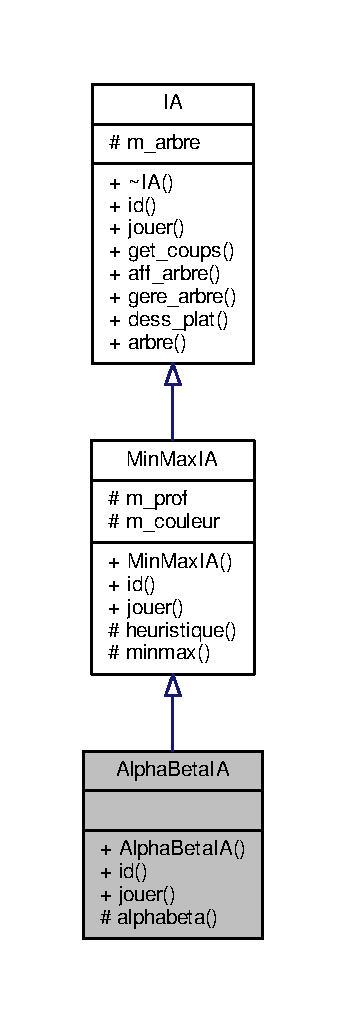
\includegraphics[width=166pt]{classAlphaBetaIA__coll__graph}
\end{center}
\end{figure}
\subsection*{Fonctions membres publiques}
\begin{DoxyCompactItemize}
\item 
{\bfseries Alpha\+Beta\+IA} (unsigned prof, C\+O\+U\+L\+E\+UR c)\hypertarget{classAlphaBetaIA_affceed21fffddfe4768ce7266810e911}{}\label{classAlphaBetaIA_affceed21fffddfe4768ce7266810e911}

\item 
virtual std\+::string \hyperlink{classAlphaBetaIA_acdf19af08e9d5c2f3fc59015e5eebf9f}{id} () const override\hypertarget{classAlphaBetaIA_acdf19af08e9d5c2f3fc59015e5eebf9f}{}\label{classAlphaBetaIA_acdf19af08e9d5c2f3fc59015e5eebf9f}

\begin{DoxyCompactList}\small\item\em Identifiant de l\textquotesingle{}\hyperlink{classIA}{IA} \+: \char`\"{}alphabeta\char`\"{}. \end{DoxyCompactList}\item 
virtual \hyperlink{structPion}{Pion} \hyperlink{classAlphaBetaIA_a33c975e65d1bec468c179972ecb1062c}{jouer} (\hyperlink{structEtat}{Etat} plateau) override\hypertarget{classAlphaBetaIA_a33c975e65d1bec468c179972ecb1062c}{}\label{classAlphaBetaIA_a33c975e65d1bec468c179972ecb1062c}

\begin{DoxyCompactList}\small\item\em Entrée de l\textquotesingle{}\hyperlink{classIA}{IA} \+: lance l\textquotesingle{}execution de l\textquotesingle{}algorithme. \end{DoxyCompactList}\end{DoxyCompactItemize}
\subsection*{Fonctions membres protégées}
\begin{DoxyCompactItemize}
\item 
virtual \hyperlink{structIA_1_1PV}{Min\+Max\+I\+A\+::\+PV} \hyperlink{classAlphaBetaIA_a864176d2e17750808299a6850f1396c3}{alphabeta} (\hyperlink{structEtat}{Etat} \&\&etat, unsigned prof, int alpha, int beta)\hypertarget{classAlphaBetaIA_a864176d2e17750808299a6850f1396c3}{}\label{classAlphaBetaIA_a864176d2e17750808299a6850f1396c3}

\begin{DoxyCompactList}\small\item\em L\textquotesingle{}algorithme en lui-\/même. \end{DoxyCompactList}\end{DoxyCompactItemize}
\subsection*{Membres hérités additionnels}


\subsection{Description détaillée}
Classe de l\textquotesingle{}\hyperlink{classIA}{IA} Alpha\+Beta Hérite de Min\+Max pour récupérer l\textquotesingle{}heuristique et la profondeur 

La documentation de cette classe a été générée à partir des fichiers suivants \+:\begin{DoxyCompactItemize}
\item 
\hyperlink{alphabetaia_8h}{alphabetaia.\+h}\item 
alphabetaia.\+cpp\end{DoxyCompactItemize}

\hypertarget{classConsole}{}\section{Référence de la classe Console}
\label{classConsole}\index{Console@{Console}}


Graphe de collaboration de Console\+:\nopagebreak
\begin{figure}[H]
\begin{center}
\leavevmode
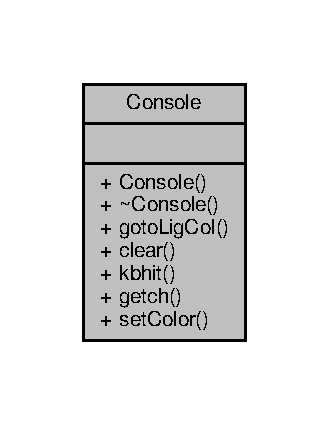
\includegraphics[width=158pt]{classConsole__coll__graph}
\end{center}
\end{figure}
\subsection*{Fonctions membres publiques}
\begin{DoxyCompactItemize}
\item 
void {\bfseries goto\+Lig\+Col} (int lig, int col)\hypertarget{classConsole_acfa13c1ba733eaa7de5182ca14a54ce1}{}\label{classConsole_acfa13c1ba733eaa7de5182ca14a54ce1}

\item 
void {\bfseries clear} ()\hypertarget{classConsole_a8b4ffaeabbea48e1f3aa1e535ee88ab8}{}\label{classConsole_a8b4ffaeabbea48e1f3aa1e535ee88ab8}

\item 
int {\bfseries kbhit} ()\hypertarget{classConsole_aae56ae7e713cb582fff7be7dd1b9f034}{}\label{classConsole_aae56ae7e713cb582fff7be7dd1b9f034}

\item 
int {\bfseries getch} ()\hypertarget{classConsole_a0fd1fe1bdd711540991cc8a19f994201}{}\label{classConsole_a0fd1fe1bdd711540991cc8a19f994201}

\item 
void {\bfseries set\+Color} (Color front=C\+O\+L\+O\+R\+\_\+\+D\+E\+F\+A\+U\+LT, Color back=C\+O\+L\+O\+R\+\_\+\+D\+E\+F\+A\+U\+L\+T\+\_\+\+B\+A\+CK)\hypertarget{classConsole_a0863977db7f233075ba98febdbcf3218}{}\label{classConsole_a0863977db7f233075ba98febdbcf3218}

\end{DoxyCompactItemize}


La documentation de cette classe a été générée à partir des fichiers suivants \+:\begin{DoxyCompactItemize}
\item 
console.\+h\item 
console.\+cpp\end{DoxyCompactItemize}

\hypertarget{structEtat}{}\section{Référence de la structure Etat}
\label{structEtat}\index{Etat@{Etat}}


Graphe de collaboration de Etat\+:\nopagebreak
\begin{figure}[H]
\begin{center}
\leavevmode
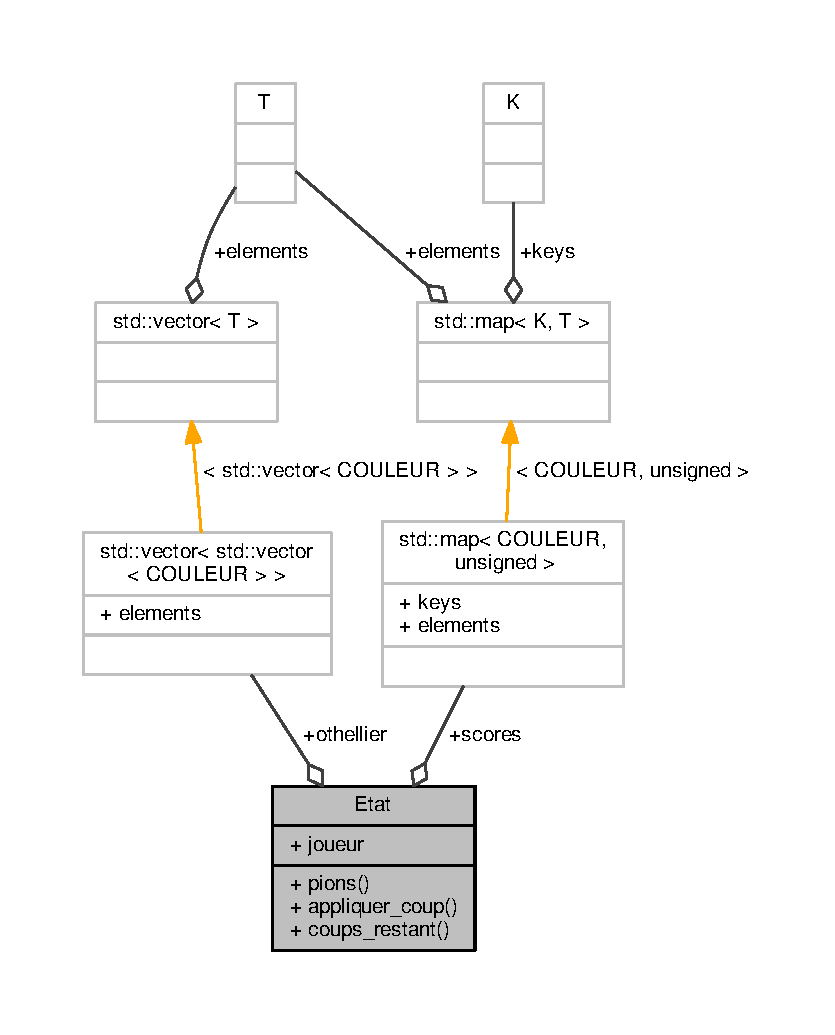
\includegraphics[width=350pt]{structEtat__coll__graph}
\end{center}
\end{figure}
\subsection*{Fonctions membres publiques}
\begin{DoxyCompactItemize}
\item 
std\+::vector$<$ \hyperlink{structPion}{Pion} $>$ {\bfseries pions} (C\+O\+U\+L\+E\+UR c) const \hypertarget{structEtat_a761f4c386924ab4216613e394184d5df}{}\label{structEtat_a761f4c386924ab4216613e394184d5df}

\item 
bool {\bfseries appliquer\+\_\+coup} (\hyperlink{structPion}{Pion} const \&p, bool fake=false)\hypertarget{structEtat_a370b369a8152ebaa56e3ceb05bde698d}{}\label{structEtat_a370b369a8152ebaa56e3ceb05bde698d}

\item 
int {\bfseries coups\+\_\+restant} (C\+O\+U\+L\+E\+UR c)\hypertarget{structEtat_a2fda3d75bfd1ed013b55d3d83409c77c}{}\label{structEtat_a2fda3d75bfd1ed013b55d3d83409c77c}

\end{DoxyCompactItemize}
\subsection*{Attributs publics}
\begin{DoxyCompactItemize}
\item 
C\+O\+U\+L\+E\+UR {\bfseries joueur}\hypertarget{structEtat_a0f6ef7f21d75e5a2c216fba4da8eadf5}{}\label{structEtat_a0f6ef7f21d75e5a2c216fba4da8eadf5}

\item 
std\+::map$<$ C\+O\+U\+L\+E\+UR, unsigned $>$ {\bfseries scores}\hypertarget{structEtat_adbf6b7995516b31b79d0f176aed8e58a}{}\label{structEtat_adbf6b7995516b31b79d0f176aed8e58a}

\item 
std\+::vector$<$ std\+::vector$<$ C\+O\+U\+L\+E\+UR $>$ $>$ {\bfseries othellier}\hypertarget{structEtat_aaeff32b606c827277a5503e05188dfa4}{}\label{structEtat_aaeff32b606c827277a5503e05188dfa4}

\end{DoxyCompactItemize}


La documentation de cette structure a été générée à partir des fichiers suivants \+:\begin{DoxyCompactItemize}
\item 
\hyperlink{etat_8h}{etat.\+h}\item 
etat.\+cpp\end{DoxyCompactItemize}

\hypertarget{classIA}{}\section{Référence de la classe IA}
\label{classIA}\index{IA@{IA}}


Graphe d\textquotesingle{}héritage de IA\+:\nopagebreak
\begin{figure}[H]
\begin{center}
\leavevmode
\includegraphics[height=550pt]{classIA__inherit__graph}
\end{center}
\end{figure}


Graphe de collaboration de IA\+:\nopagebreak
\begin{figure}[H]
\begin{center}
\leavevmode
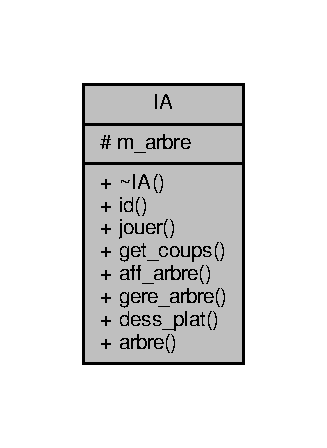
\includegraphics[width=157pt]{classIA__coll__graph}
\end{center}
\end{figure}
\subsection*{Classes}
\begin{DoxyCompactItemize}
\item 
struct \hyperlink{structIA_1_1PV}{PV}
\end{DoxyCompactItemize}
\subsection*{Fonctions membres publiques}
\begin{DoxyCompactItemize}
\item 
virtual std\+::string {\bfseries id} () const =0\hypertarget{classIA_a766f10d2cd5450868523e2fa184fdf93}{}\label{classIA_a766f10d2cd5450868523e2fa184fdf93}

\item 
virtual \hyperlink{structPion}{Pion} {\bfseries jouer} (\hyperlink{structEtat}{Etat} plateau)=0\hypertarget{classIA_a3f40133e71c6bbe7fe7c72b4792dccb4}{}\label{classIA_a3f40133e71c6bbe7fe7c72b4792dccb4}

\item 
std\+::set$<$ \hyperlink{structPion}{Pion}, bool(\&)(\hyperlink{structPion}{Pion} const \&, \hyperlink{structPion}{Pion} const \&)$>$ {\bfseries get\+\_\+coups} (\hyperlink{structEtat}{Etat} const \&plateau) const \hypertarget{classIA_a6a1a014ffa6b3dbf6c1f401ecfa55148}{}\label{classIA_a6a1a014ffa6b3dbf6c1f401ecfa55148}

\item 
void {\bfseries aff\+\_\+arbre} (\hyperlink{classConsole}{Console} $\ast$s\+\_\+console, std\+::shared\+\_\+ptr$<$ \hyperlink{classNoeud}{Noeud}$<$ \hyperlink{structIA_1_1PV}{PV} $>$$>$ noeud, int num\+\_\+coup)\hypertarget{classIA_aca13a5971e87f358cd9e70188448b698}{}\label{classIA_aca13a5971e87f358cd9e70188448b698}

\item 
bool {\bfseries gere\+\_\+arbre} (\hyperlink{classConsole}{Console} $\ast$s\+\_\+console, std\+::shared\+\_\+ptr$<$ \hyperlink{classNoeud}{Noeud}$<$ \hyperlink{structIA_1_1PV}{PV} $>$$>$ noeud, int num\+\_\+coup, std\+::vector$<$ std\+::vector$<$ C\+O\+U\+L\+E\+UR $>$$>$ othellier)\hypertarget{classIA_aa2896700500f380a77b8efc6dff9ed5e}{}\label{classIA_aa2896700500f380a77b8efc6dff9ed5e}

\item 
void {\bfseries dess\+\_\+plat} (\hyperlink{classConsole}{Console} $\ast$s\+\_\+console, int x, int y, \hyperlink{structPion}{Pion} pion, std\+::vector$<$ std\+::vector$<$ C\+O\+U\+L\+E\+UR $>$$>$ othellier, int val)\hypertarget{classIA_a2bb3de5d20fb887a3e88d6b0d698c381}{}\label{classIA_a2bb3de5d20fb887a3e88d6b0d698c381}

\item 
std\+::shared\+\_\+ptr$<$ \hyperlink{classNoeud}{Noeud}$<$ \hyperlink{structIA_1_1PV}{PV} $>$ $>$ {\bfseries arbre} () const \hypertarget{classIA_a27c2b1942849e7fbd4c77f4c0fa0d88d}{}\label{classIA_a27c2b1942849e7fbd4c77f4c0fa0d88d}

\end{DoxyCompactItemize}
\subsection*{Attributs protégés}
\begin{DoxyCompactItemize}
\item 
std\+::shared\+\_\+ptr$<$ \hyperlink{classNoeud}{Noeud}$<$ \hyperlink{structIA_1_1PV}{PV} $>$ $>$ {\bfseries m\+\_\+arbre}\hypertarget{classIA_a6666e00b08d090ab464d1847c6b9db32}{}\label{classIA_a6666e00b08d090ab464d1847c6b9db32}

\end{DoxyCompactItemize}


La documentation de cette classe a été générée à partir des fichiers suivants \+:\begin{DoxyCompactItemize}
\item 
ia.\+h\item 
ia.\+cpp\end{DoxyCompactItemize}

\hypertarget{classMemArbre}{}\section{Référence de la classe Mem\+Arbre}
\label{classMemArbre}\index{Mem\+Arbre@{Mem\+Arbre}}


Graphe d\textquotesingle{}héritage de Mem\+Arbre\+:\nopagebreak
\begin{figure}[H]
\begin{center}
\leavevmode
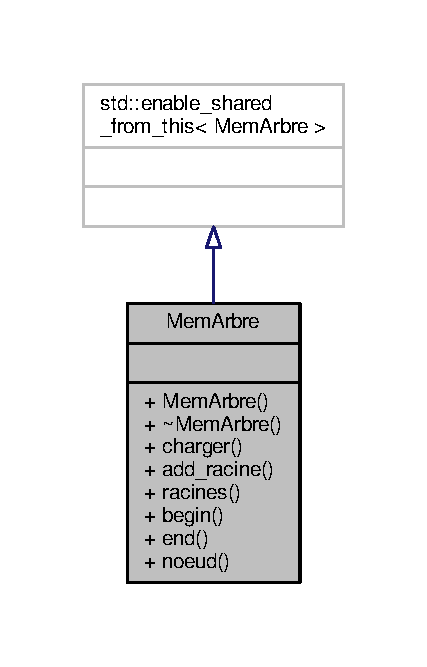
\includegraphics[width=205pt]{classMemArbre__inherit__graph}
\end{center}
\end{figure}


Graphe de collaboration de Mem\+Arbre\+:\nopagebreak
\begin{figure}[H]
\begin{center}
\leavevmode
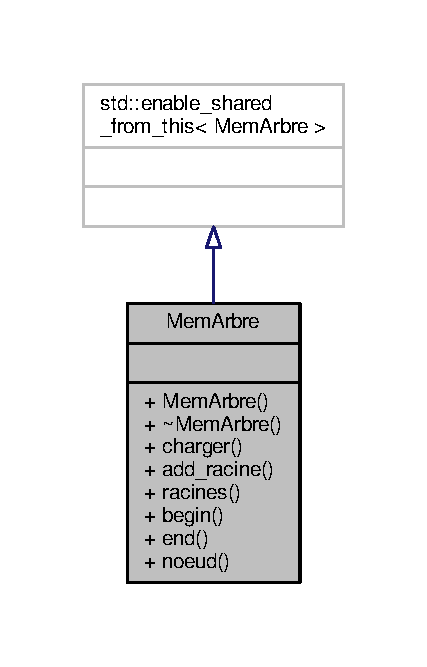
\includegraphics[width=205pt]{classMemArbre__coll__graph}
\end{center}
\end{figure}
\subsection*{Classes}
\begin{DoxyCompactItemize}
\item 
class \hyperlink{classMemArbre_1_1Noeud}{Noeud}
\end{DoxyCompactItemize}
\subsection*{Types publics}
\begin{DoxyCompactItemize}
\item 
using {\bfseries iterateur} = std\+::map$<$ int, std\+::shared\+\_\+ptr$<$ \hyperlink{classMemArbre_1_1Noeud}{Noeud} $>$$>$\+::const\+\_\+iterator\hypertarget{classMemArbre_a4f15f8cc13e7c9e0909b803e6d995cac}{}\label{classMemArbre_a4f15f8cc13e7c9e0909b803e6d995cac}

\end{DoxyCompactItemize}
\subsection*{Fonctions membres publiques}
\begin{DoxyCompactItemize}
\item 
{\bfseries Mem\+Arbre} (std\+::string const \&fichier)\hypertarget{classMemArbre_ac5190591ba7c14a65a0c4dac3b79dfd7}{}\label{classMemArbre_ac5190591ba7c14a65a0c4dac3b79dfd7}

\item 
void \hyperlink{classMemArbre_aed29ba0b60d2b1000df67bcc8c20017f}{charger} ()\hypertarget{classMemArbre_aed29ba0b60d2b1000df67bcc8c20017f}{}\label{classMemArbre_aed29ba0b60d2b1000df67bcc8c20017f}

\begin{DoxyCompactList}\small\item\em Lance le chargement de l\textquotesingle{}arbre. \end{DoxyCompactList}\item 
std\+::shared\+\_\+ptr$<$ \hyperlink{classMemArbre_1_1Noeud}{Noeud} $>$ \hyperlink{classMemArbre_ac18d57ffee484bf225255213ba5b0cbe}{add\+\_\+racine} (int val, std\+::tuple$<$ int, int $>$ const \&coords)\hypertarget{classMemArbre_ac18d57ffee484bf225255213ba5b0cbe}{}\label{classMemArbre_ac18d57ffee484bf225255213ba5b0cbe}

\begin{DoxyCompactList}\small\item\em ajoute une racine au fichier \end{DoxyCompactList}\item 
std\+::set$<$ std\+::shared\+\_\+ptr$<$ \hyperlink{classMemArbre_1_1Noeud}{Noeud} $>$ $>$ \hyperlink{classMemArbre_a5e84dc402d7e740f853cef4107f7cce4}{racines} () const \hypertarget{classMemArbre_a5e84dc402d7e740f853cef4107f7cce4}{}\label{classMemArbre_a5e84dc402d7e740f853cef4107f7cce4}

\begin{DoxyCompactList}\small\item\em Renvoie les racines. \end{DoxyCompactList}\item 
iterateur {\bfseries begin} () const \hypertarget{classMemArbre_afd69fc6c9f2fe86ac9dea7e4ca4223e0}{}\label{classMemArbre_afd69fc6c9f2fe86ac9dea7e4ca4223e0}

\item 
iterateur {\bfseries end} () const \hypertarget{classMemArbre_a87f7bbf0ea68be14aa83661585bcf4a8}{}\label{classMemArbre_a87f7bbf0ea68be14aa83661585bcf4a8}

\item 
std\+::shared\+\_\+ptr$<$ \hyperlink{classMemArbre_1_1Noeud}{Noeud} $>$ \hyperlink{classMemArbre_a474515fbd83097859ff121dd0cc4a57c}{noeud} (int pos) const \hypertarget{classMemArbre_a474515fbd83097859ff121dd0cc4a57c}{}\label{classMemArbre_a474515fbd83097859ff121dd0cc4a57c}

\begin{DoxyCompactList}\small\item\em Renvoie le noeud à la position donnée. \end{DoxyCompactList}\end{DoxyCompactItemize}


La documentation de cette classe a été générée à partir des fichiers suivants \+:\begin{DoxyCompactItemize}
\item 
memarbre.\+h\item 
memarbre.\+cpp\end{DoxyCompactItemize}

\hypertarget{classMemIA}{}\section{Référence de la classe Mem\+IA}
\label{classMemIA}\index{Mem\+IA@{Mem\+IA}}


Graphe d\textquotesingle{}héritage de Mem\+IA\+:\nopagebreak
\begin{figure}[H]
\begin{center}
\leavevmode
\includegraphics[height=550pt]{classMemIA__inherit__graph}
\end{center}
\end{figure}


Graphe de collaboration de Mem\+IA\+:\nopagebreak
\begin{figure}[H]
\begin{center}
\leavevmode
\includegraphics[height=550pt]{classMemIA__coll__graph}
\end{center}
\end{figure}
\subsection*{Fonctions membres publiques}
\begin{DoxyCompactItemize}
\item 
{\bfseries Mem\+IA} (std\+::string const \&fichier, unsigned prof, C\+O\+U\+L\+E\+UR c)\hypertarget{classMemIA_a2c0eed85d2e17e428b62fb4ba23cde1c}{}\label{classMemIA_a2c0eed85d2e17e428b62fb4ba23cde1c}

\item 
virtual std\+::string \hyperlink{classMemIA_a1075fe7a51c71bca7fd6b3cd63d3271d}{id} () const override\hypertarget{classMemIA_a1075fe7a51c71bca7fd6b3cd63d3271d}{}\label{classMemIA_a1075fe7a51c71bca7fd6b3cd63d3271d}

\begin{DoxyCompactList}\small\item\em Identifiant de l\textquotesingle{}\hyperlink{classIA}{IA} \+: \char`\"{}alphabeta\char`\"{}. \end{DoxyCompactList}\item 
virtual \hyperlink{structPion}{Pion} \hyperlink{classMemIA_a82b883399e9d663c382994190572c0a6}{jouer} (\hyperlink{structEtat}{Etat} plateau) override\hypertarget{classMemIA_a82b883399e9d663c382994190572c0a6}{}\label{classMemIA_a82b883399e9d663c382994190572c0a6}

\begin{DoxyCompactList}\small\item\em Entrée de l\textquotesingle{}\hyperlink{classIA}{IA} \+: lance l\textquotesingle{}execution de l\textquotesingle{}algorithme. \end{DoxyCompactList}\item 
void {\bfseries gagne} ()\hypertarget{classMemIA_a5c2b4334f3830d2659d4b25d174aa563}{}\label{classMemIA_a5c2b4334f3830d2659d4b25d174aa563}

\item 
void {\bfseries perdu} ()\hypertarget{classMemIA_a1aba65e04d27d75f0dee1f53d9f20025}{}\label{classMemIA_a1aba65e04d27d75f0dee1f53d9f20025}

\item 
void {\bfseries set\+\_\+prof} (unsigned prof)\hypertarget{classMemIA_a533276bc61af601452e9b1c29953371d}{}\label{classMemIA_a533276bc61af601452e9b1c29953371d}

\item 
void {\bfseries set\+\_\+noeud} (int pos)\hypertarget{classMemIA_a4efede59191924b76042bbc45860efc6}{}\label{classMemIA_a4efede59191924b76042bbc45860efc6}

\end{DoxyCompactItemize}
\subsection*{Membres hérités additionnels}


La documentation de cette classe a été générée à partir des fichiers suivants \+:\begin{DoxyCompactItemize}
\item 
memia.\+h\item 
memia.\+cpp\end{DoxyCompactItemize}

\hypertarget{classMenu}{}\section{Référence de la classe Menu}
\label{classMenu}\index{Menu@{Menu}}


Graphe de collaboration de Menu\+:\nopagebreak
\begin{figure}[H]
\begin{center}
\leavevmode
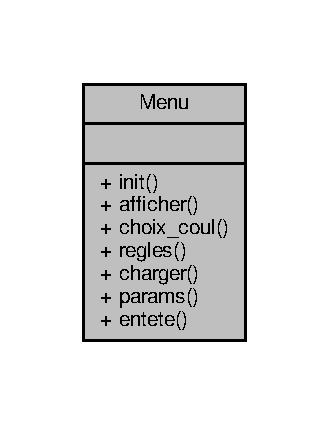
\includegraphics[width=158pt]{classMenu__coll__graph}
\end{center}
\end{figure}
\subsection*{Fonctions membres publiques}
\begin{DoxyCompactItemize}
\item 
int {\bfseries init} ()\hypertarget{classMenu_a514c26765dc9e00098f199c6c98788a4}{}\label{classMenu_a514c26765dc9e00098f199c6c98788a4}

\item 
void {\bfseries afficher} ()\hypertarget{classMenu_afc925fd19c50c3c724924f32673fbaf8}{}\label{classMenu_afc925fd19c50c3c724924f32673fbaf8}

\item 
C\+O\+U\+L\+E\+UR {\bfseries choix\+\_\+coul} () const \hypertarget{classMenu_a8985cbb2c3618edc7c4c42eb94ef9513}{}\label{classMenu_a8985cbb2c3618edc7c4c42eb94ef9513}

\item 
void {\bfseries regles} () const \hypertarget{classMenu_abca65b44c7a2f424a00c4381f853dee0}{}\label{classMenu_abca65b44c7a2f424a00c4381f853dee0}

\item 
bool {\bfseries charger} (\hyperlink{classTableau}{Tableau} \&tab, bool \&memia\+\_\+noire, bool \&memia\+\_\+blanche) const \hypertarget{classMenu_a4d938d0f79289ad48576d7a99db0461d}{}\label{classMenu_a4d938d0f79289ad48576d7a99db0461d}

\item 
void {\bfseries params} ()\hypertarget{classMenu_aceb88979ec505e8aba9924dc8206678c}{}\label{classMenu_aceb88979ec505e8aba9924dc8206678c}

\end{DoxyCompactItemize}
\subsection*{Fonctions membres publiques statiques}
\begin{DoxyCompactItemize}
\item 
static void {\bfseries entete} ()\hypertarget{classMenu_a7f575e5c439d03cef1e1a5a79a66aa54}{}\label{classMenu_a7f575e5c439d03cef1e1a5a79a66aa54}

\end{DoxyCompactItemize}


La documentation de cette classe a été générée à partir des fichiers suivants \+:\begin{DoxyCompactItemize}
\item 
menu.\+h\item 
menu.\+cpp\end{DoxyCompactItemize}

\hypertarget{classMinMaxIA}{}\section{Référence de la classe Min\+Max\+IA}
\label{classMinMaxIA}\index{Min\+Max\+IA@{Min\+Max\+IA}}


Graphe d\textquotesingle{}héritage de Min\+Max\+IA\+:\nopagebreak
\begin{figure}[H]
\begin{center}
\leavevmode
\includegraphics[height=550pt]{classMinMaxIA__inherit__graph}
\end{center}
\end{figure}


Graphe de collaboration de Min\+Max\+IA\+:\nopagebreak
\begin{figure}[H]
\begin{center}
\leavevmode
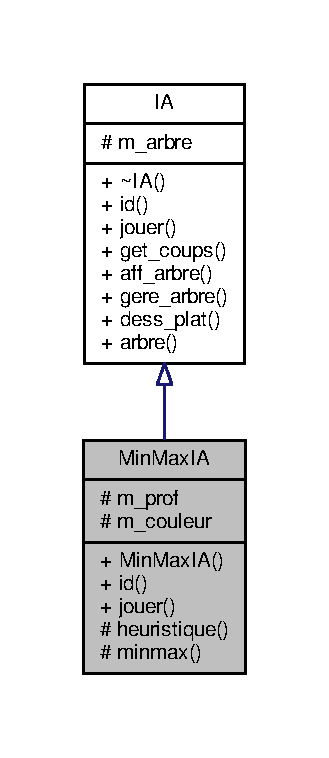
\includegraphics[width=158pt]{classMinMaxIA__coll__graph}
\end{center}
\end{figure}
\subsection*{Fonctions membres publiques}
\begin{DoxyCompactItemize}
\item 
{\bfseries Min\+Max\+IA} (unsigned prof, C\+O\+U\+L\+E\+UR c)\hypertarget{classMinMaxIA_ab186638b8bf69698b86415555734a926}{}\label{classMinMaxIA_ab186638b8bf69698b86415555734a926}

\item 
virtual std\+::string {\bfseries id} () const override\hypertarget{classMinMaxIA_ace6db5b6ab7a0aaba72d2bf16a44f6f3}{}\label{classMinMaxIA_ace6db5b6ab7a0aaba72d2bf16a44f6f3}

\item 
virtual \hyperlink{structPion}{Pion} {\bfseries jouer} (\hyperlink{structEtat}{Etat} plateau) override\hypertarget{classMinMaxIA_a829500a59568c81e902862933e4f9931}{}\label{classMinMaxIA_a829500a59568c81e902862933e4f9931}

\end{DoxyCompactItemize}
\subsection*{Fonctions membres protégées}
\begin{DoxyCompactItemize}
\item 
virtual int {\bfseries heuristique} (\hyperlink{structEtat}{Etat} \&\&etat) final\hypertarget{classMinMaxIA_a3261d2cb9a7105d930a0e67722f4289f}{}\label{classMinMaxIA_a3261d2cb9a7105d930a0e67722f4289f}

\item 
virtual \hyperlink{structIA_1_1PV}{PV} {\bfseries minmax} (\hyperlink{structEtat}{Etat} \&\&etat, unsigned prof, std\+::shared\+\_\+ptr$<$ \hyperlink{classNoeud}{Noeud}$<$ \hyperlink{structIA_1_1PV}{PV} $>$$>$ noeud)\hypertarget{classMinMaxIA_a15caae3b6117d717bb6c72dd97acc7c6}{}\label{classMinMaxIA_a15caae3b6117d717bb6c72dd97acc7c6}

\end{DoxyCompactItemize}
\subsection*{Attributs protégés}
\begin{DoxyCompactItemize}
\item 
unsigned {\bfseries m\+\_\+prof}\hypertarget{classMinMaxIA_aab16a043c48ab6b300cdabf8d67c32ec}{}\label{classMinMaxIA_aab16a043c48ab6b300cdabf8d67c32ec}

\item 
C\+O\+U\+L\+E\+UR {\bfseries m\+\_\+couleur}\hypertarget{classMinMaxIA_a9dd148bfadb7fd84d7392ece6669d841}{}\label{classMinMaxIA_a9dd148bfadb7fd84d7392ece6669d841}

\end{DoxyCompactItemize}


La documentation de cette classe a été générée à partir des fichiers suivants \+:\begin{DoxyCompactItemize}
\item 
minmaxia.\+h\item 
minmaxia.\+cpp\end{DoxyCompactItemize}

\hypertarget{classNegaMaxIA}{}\section{Référence de la classe Nega\+Max\+IA}
\label{classNegaMaxIA}\index{Nega\+Max\+IA@{Nega\+Max\+IA}}


Graphe d\textquotesingle{}héritage de Nega\+Max\+IA\+:\nopagebreak
\begin{figure}[H]
\begin{center}
\leavevmode
\includegraphics[height=550pt]{classNegaMaxIA__inherit__graph}
\end{center}
\end{figure}


Graphe de collaboration de Nega\+Max\+IA\+:\nopagebreak
\begin{figure}[H]
\begin{center}
\leavevmode
\includegraphics[height=550pt]{classNegaMaxIA__coll__graph}
\end{center}
\end{figure}
\subsection*{Fonctions membres publiques}
\begin{DoxyCompactItemize}
\item 
{\bfseries Nega\+Max\+IA} (unsigned prof, C\+O\+U\+L\+E\+UR c)\hypertarget{classNegaMaxIA_a3fd21d1bc1f35237509452d3e3ec2468}{}\label{classNegaMaxIA_a3fd21d1bc1f35237509452d3e3ec2468}

\item 
virtual std\+::string \hyperlink{classNegaMaxIA_aa8b42b9e3740f6df0d77fbf44d9062f4}{id} () const override\hypertarget{classNegaMaxIA_aa8b42b9e3740f6df0d77fbf44d9062f4}{}\label{classNegaMaxIA_aa8b42b9e3740f6df0d77fbf44d9062f4}

\begin{DoxyCompactList}\small\item\em Identifiant de l\textquotesingle{}\hyperlink{classIA}{IA} \+: \char`\"{}alphabeta\char`\"{}. \end{DoxyCompactList}\end{DoxyCompactItemize}
\subsection*{Fonctions membres protégées}
\begin{DoxyCompactItemize}
\item 
virtual \hyperlink{structIA_1_1PV}{Min\+Max\+I\+A\+::\+PV} \hyperlink{classNegaMaxIA_afe019dd4570ec304b9b6b9c56596a51a}{alphabeta} (\hyperlink{structEtat}{Etat} \&\&etat, unsigned prof, int alpha, int beta) override\hypertarget{classNegaMaxIA_afe019dd4570ec304b9b6b9c56596a51a}{}\label{classNegaMaxIA_afe019dd4570ec304b9b6b9c56596a51a}

\begin{DoxyCompactList}\small\item\em L\textquotesingle{}algorithme en lui-\/même. \end{DoxyCompactList}\end{DoxyCompactItemize}
\subsection*{Membres hérités additionnels}


La documentation de cette classe a été générée à partir des fichiers suivants \+:\begin{DoxyCompactItemize}
\item 
negamaxia.\+h\item 
negamaxia.\+cpp\end{DoxyCompactItemize}

\hypertarget{classNoeud}{}\section{Référence du modèle de la classe Noeud$<$ T $>$}
\label{classNoeud}\index{Noeud$<$ T $>$@{Noeud$<$ T $>$}}


Graphe d\textquotesingle{}héritage de Noeud$<$ T $>$\+:\nopagebreak
\begin{figure}[H]
\begin{center}
\leavevmode
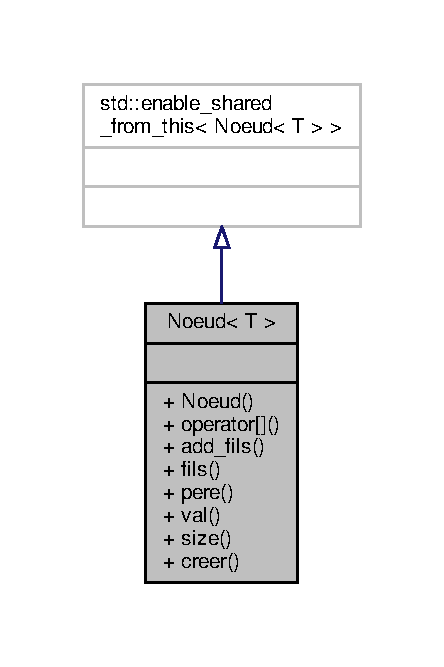
\includegraphics[width=213pt]{classNoeud__inherit__graph}
\end{center}
\end{figure}


Graphe de collaboration de Noeud$<$ T $>$\+:\nopagebreak
\begin{figure}[H]
\begin{center}
\leavevmode
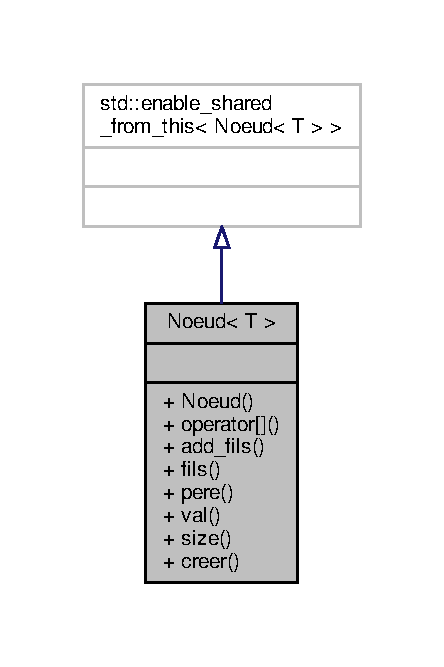
\includegraphics[width=213pt]{classNoeud__coll__graph}
\end{center}
\end{figure}
\subsection*{Fonctions membres publiques}
\begin{DoxyCompactItemize}
\item 
{\bfseries Noeud} (T const \&val, std\+::weak\+\_\+ptr$<$ \hyperlink{classNoeud}{Noeud}$<$ T $>$$>$ const \&pere)\hypertarget{classNoeud_a1da54304cf1cb3ef8b185fddb392958a}{}\label{classNoeud_a1da54304cf1cb3ef8b185fddb392958a}

\item 
\hyperlink{classNoeud}{Noeud}$<$ T $>$ {\bfseries operator\mbox{[}$\,$\mbox{]}} (int i)\hypertarget{classNoeud_ac15ebbd02aaff1c7ea6238617431e11f}{}\label{classNoeud_ac15ebbd02aaff1c7ea6238617431e11f}

\item 
std\+::shared\+\_\+ptr$<$ \hyperlink{classNoeud}{Noeud}$<$ T $>$ $>$ {\bfseries add\+\_\+fils} (T const \&val)\hypertarget{classNoeud_a6a494c4a2e3d844addfd3af6e65d527d}{}\label{classNoeud_a6a494c4a2e3d844addfd3af6e65d527d}

\item 
std\+::shared\+\_\+ptr$<$ \hyperlink{classNoeud}{Noeud}$<$ T $>$ $>$ {\bfseries fils} (int i)\hypertarget{classNoeud_ae968b7fe5d1c060ff61e8ab383a106b8}{}\label{classNoeud_ae968b7fe5d1c060ff61e8ab383a106b8}

\item 
std\+::shared\+\_\+ptr$<$ \hyperlink{classNoeud}{Noeud}$<$ T $>$ $>$ {\bfseries pere} ()\hypertarget{classNoeud_a226193dbebac6cf5e8bd55bf47f6bf75}{}\label{classNoeud_a226193dbebac6cf5e8bd55bf47f6bf75}

\item 
std\+::add\+\_\+lvalue\+\_\+reference$<$ T $>$\+::type {\bfseries val} ()\hypertarget{classNoeud_a76f29413cf4c786bb1aa8be13aed2276}{}\label{classNoeud_a76f29413cf4c786bb1aa8be13aed2276}

\item 
unsigned {\bfseries size} () const \hypertarget{classNoeud_a8b1d01e51a0917ec172d57c2afa2f31c}{}\label{classNoeud_a8b1d01e51a0917ec172d57c2afa2f31c}

\end{DoxyCompactItemize}
\subsection*{Fonctions membres publiques statiques}
\begin{DoxyCompactItemize}
\item 
static std\+::shared\+\_\+ptr$<$ \hyperlink{classNoeud}{Noeud}$<$ T $>$ $>$ {\bfseries creer} (T const \&val)\hypertarget{classNoeud_a53503e6bae571316d778c39214693710}{}\label{classNoeud_a53503e6bae571316d778c39214693710}

\end{DoxyCompactItemize}


La documentation de cette classe a été générée à partir du fichier suivant \+:\begin{DoxyCompactItemize}
\item 
noeud.\+h\end{DoxyCompactItemize}

\hypertarget{classMemArbre_1_1Noeud}{}\section{Référence de la classe Mem\+Arbre\+:\+:Noeud}
\label{classMemArbre_1_1Noeud}\index{Mem\+Arbre\+::\+Noeud@{Mem\+Arbre\+::\+Noeud}}


Graphe d\textquotesingle{}héritage de Mem\+Arbre\+:\+:Noeud\+:\nopagebreak
\begin{figure}[H]
\begin{center}
\leavevmode
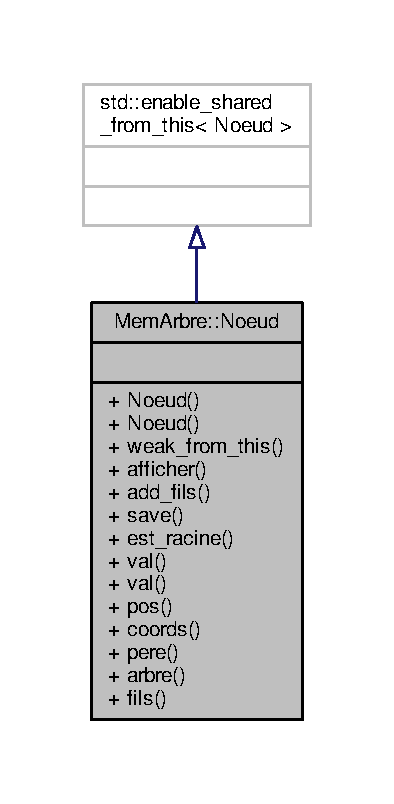
\includegraphics[width=189pt]{classMemArbre_1_1Noeud__inherit__graph}
\end{center}
\end{figure}


Graphe de collaboration de Mem\+Arbre\+:\+:Noeud\+:\nopagebreak
\begin{figure}[H]
\begin{center}
\leavevmode
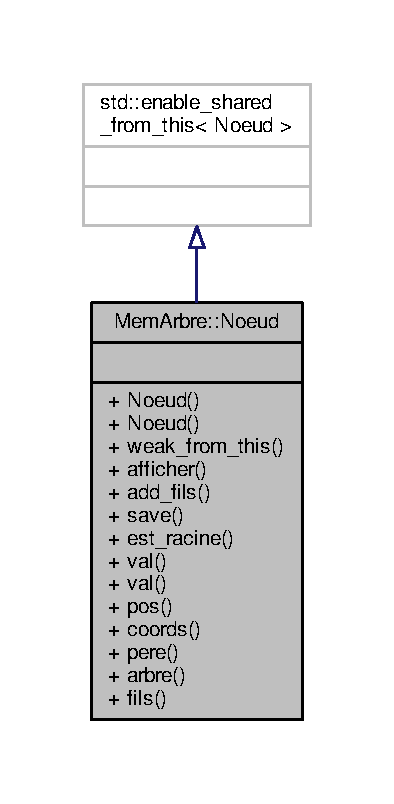
\includegraphics[width=189pt]{classMemArbre_1_1Noeud__coll__graph}
\end{center}
\end{figure}
\subsection*{Fonctions membres publiques}
\begin{DoxyCompactItemize}
\item 
{\bfseries Noeud} (int val, std\+::tuple$<$ int, int $>$ const \&coords, int pos, std\+::shared\+\_\+ptr$<$ \hyperlink{classMemArbre}{Mem\+Arbre} $>$ const \&arbre)\hypertarget{classMemArbre_1_1Noeud_a8fb60f07cdaa6c159102b5c28ccd904f}{}\label{classMemArbre_1_1Noeud_a8fb60f07cdaa6c159102b5c28ccd904f}

\item 
{\bfseries Noeud} (int val, std\+::tuple$<$ int, int $>$ const \&coords, int pos, std\+::shared\+\_\+ptr$<$ \hyperlink{classMemArbre}{Mem\+Arbre} $>$ const \&arbre, std\+::shared\+\_\+ptr$<$ \hyperlink{classMemArbre_1_1Noeud}{Noeud} $>$ const \&pere)\hypertarget{classMemArbre_1_1Noeud_a96ab7701e3ac3a755c66e2332f69cd7d}{}\label{classMemArbre_1_1Noeud_a96ab7701e3ac3a755c66e2332f69cd7d}

\item 
std\+::weak\+\_\+ptr$<$ \hyperlink{classMemArbre_1_1Noeud}{Noeud} $>$ \hyperlink{classMemArbre_1_1Noeud_a4639b419945fdb26f7ba9c967559bcf3}{weak\+\_\+from\+\_\+this} ()\hypertarget{classMemArbre_1_1Noeud_a4639b419945fdb26f7ba9c967559bcf3}{}\label{classMemArbre_1_1Noeud_a4639b419945fdb26f7ba9c967559bcf3}

\begin{DoxyCompactList}\small\item\em Renvoie un weak\+\_\+ptr sur this. \end{DoxyCompactList}\item 
std\+::ostream \& \hyperlink{classMemArbre_1_1Noeud_ae5c5794ad07ff855c5e472f10c890c38}{afficher} (std\+::ostream \&stream) const \hypertarget{classMemArbre_1_1Noeud_ae5c5794ad07ff855c5e472f10c890c38}{}\label{classMemArbre_1_1Noeud_ae5c5794ad07ff855c5e472f10c890c38}

\begin{DoxyCompactList}\small\item\em Permet d\textquotesingle{}afficher le noeud. \end{DoxyCompactList}\item 
std\+::shared\+\_\+ptr$<$ \hyperlink{classMemArbre_1_1Noeud}{Noeud} $>$ \hyperlink{classMemArbre_1_1Noeud_a738b4af9c935bc05dac33f4c48bed0cf}{add\+\_\+fils} (int val, std\+::tuple$<$ int, int $>$ const \&coords)\hypertarget{classMemArbre_1_1Noeud_a738b4af9c935bc05dac33f4c48bed0cf}{}\label{classMemArbre_1_1Noeud_a738b4af9c935bc05dac33f4c48bed0cf}

\begin{DoxyCompactList}\small\item\em Crée un fils avec la valeur et la coordonnée données. \end{DoxyCompactList}\item 
void \hyperlink{classMemArbre_1_1Noeud_a710f476869b71d13a8e26eddd86a08f9}{save} ()\hypertarget{classMemArbre_1_1Noeud_a710f476869b71d13a8e26eddd86a08f9}{}\label{classMemArbre_1_1Noeud_a710f476869b71d13a8e26eddd86a08f9}

\begin{DoxyCompactList}\small\item\em Sauvegarde le noeud dans le fichier. \end{DoxyCompactList}\item 
bool \hyperlink{classMemArbre_1_1Noeud_abb962cfea5c62f59b00ba4d89be3bee9}{est\+\_\+racine} () const \hypertarget{classMemArbre_1_1Noeud_abb962cfea5c62f59b00ba4d89be3bee9}{}\label{classMemArbre_1_1Noeud_abb962cfea5c62f59b00ba4d89be3bee9}

\begin{DoxyCompactList}\small\item\em Renvoie vrai si le noeud est une racine. \end{DoxyCompactList}\item 
int {\bfseries val} () const \hypertarget{classMemArbre_1_1Noeud_a6a4ea4e942bf9386355fbc07b9b20a58}{}\label{classMemArbre_1_1Noeud_a6a4ea4e942bf9386355fbc07b9b20a58}

\item 
void {\bfseries val} (int val)\hypertarget{classMemArbre_1_1Noeud_a1a0284e4bbece82e6ba90147daf15fbb}{}\label{classMemArbre_1_1Noeud_a1a0284e4bbece82e6ba90147daf15fbb}

\item 
int const \& {\bfseries pos} () const \hypertarget{classMemArbre_1_1Noeud_a80908f07b60962b3ad38a5bcdd3e739f}{}\label{classMemArbre_1_1Noeud_a80908f07b60962b3ad38a5bcdd3e739f}

\item 
std\+::tuple$<$ int, int $>$ \& {\bfseries coords} ()\hypertarget{classMemArbre_1_1Noeud_a97ffd0d907bf6d61fc19446212c676de}{}\label{classMemArbre_1_1Noeud_a97ffd0d907bf6d61fc19446212c676de}

\item 
std\+::shared\+\_\+ptr$<$ \hyperlink{classMemArbre_1_1Noeud}{Noeud} $>$ {\bfseries pere} () const \hypertarget{classMemArbre_1_1Noeud_ade2357880c5929f836edc962301edf25}{}\label{classMemArbre_1_1Noeud_ade2357880c5929f836edc962301edf25}

\item 
std\+::shared\+\_\+ptr$<$ \hyperlink{classMemArbre}{Mem\+Arbre} $>$ {\bfseries arbre} () const \hypertarget{classMemArbre_1_1Noeud_a3e4c43603bc73e9b3c59c4f484d66436}{}\label{classMemArbre_1_1Noeud_a3e4c43603bc73e9b3c59c4f484d66436}

\item 
std\+::set$<$ std\+::shared\+\_\+ptr$<$ \hyperlink{classMemArbre_1_1Noeud}{Noeud} $>$ $>$ const \& {\bfseries fils} () const \hypertarget{classMemArbre_1_1Noeud_a7c627d3c87dac568a9d39d8f65516626}{}\label{classMemArbre_1_1Noeud_a7c627d3c87dac568a9d39d8f65516626}

\end{DoxyCompactItemize}
\subsection*{Amis}
\begin{DoxyCompactItemize}
\item 
class {\bfseries Mem\+Arbre}\hypertarget{classMemArbre_1_1Noeud_a2828cd0bf50a0db376c8e9b9eeda2637}{}\label{classMemArbre_1_1Noeud_a2828cd0bf50a0db376c8e9b9eeda2637}

\end{DoxyCompactItemize}


La documentation de cette classe a été générée à partir des fichiers suivants \+:\begin{DoxyCompactItemize}
\item 
memarbre.\+h\item 
memarbre.\+cpp\end{DoxyCompactItemize}

\hypertarget{structP}{}\section{Référence de la structure P}
\label{structP}\index{P@{P}}


Graphe de collaboration de P\+:\nopagebreak
\begin{figure}[H]
\begin{center}
\leavevmode
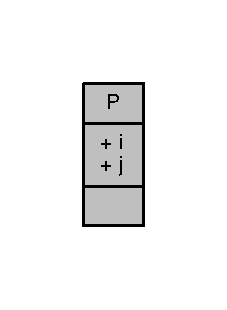
\includegraphics[width=109pt]{structP__coll__graph}
\end{center}
\end{figure}
\subsection*{Attributs publics}
\begin{DoxyCompactItemize}
\item 
int {\bfseries i}\hypertarget{structP_a529b8eb5e5e9de9bbfa1ace78d7c6a39}{}\label{structP_a529b8eb5e5e9de9bbfa1ace78d7c6a39}

\item 
int {\bfseries j}\hypertarget{structP_a2a742a8540f2aa8b480c4def50e4edd0}{}\label{structP_a2a742a8540f2aa8b480c4def50e4edd0}

\end{DoxyCompactItemize}


La documentation de cette structure a été générée à partir du fichier suivant \+:\begin{DoxyCompactItemize}
\item 
etat.\+cpp\end{DoxyCompactItemize}

\hypertarget{structPion}{}\section{Référence de la structure Pion}
\label{structPion}\index{Pion@{Pion}}


Structure de \hyperlink{structPion}{Pion}.  




{\ttfamily \#include $<$pion.\+h$>$}



Graphe de collaboration de Pion\+:\nopagebreak
\begin{figure}[H]
\begin{center}
\leavevmode
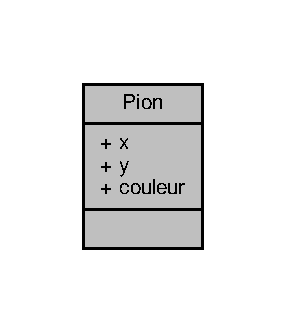
\includegraphics[width=137pt]{structPion__coll__graph}
\end{center}
\end{figure}
\subsection*{Attributs publics}
\begin{DoxyCompactItemize}
\item 
int {\bfseries x}\hypertarget{structPion_af6505c8de5ccc06d564945534272694c}{}\label{structPion_af6505c8de5ccc06d564945534272694c}

\item 
int {\bfseries y}\hypertarget{structPion_aa7fb8d98415132074045e4aebf7d97dd}{}\label{structPion_aa7fb8d98415132074045e4aebf7d97dd}

\item 
C\+O\+U\+L\+E\+UR {\bfseries couleur}\hypertarget{structPion_a1bb174054b197226d0c44f4a2920e409}{}\label{structPion_a1bb174054b197226d0c44f4a2920e409}

\end{DoxyCompactItemize}


\subsection{Description détaillée}
Structure de \hyperlink{structPion}{Pion}. 

La documentation de cette structure a été générée à partir du fichier suivant \+:\begin{DoxyCompactItemize}
\item 
pion.\+h\end{DoxyCompactItemize}

\hypertarget{structIA_1_1PV}{}\section{Référence de la structure IA\+:\+:PV}
\label{structIA_1_1PV}\index{I\+A\+::\+PV@{I\+A\+::\+PV}}


Graphe de collaboration de IA\+:\+:PV\+:\nopagebreak
\begin{figure}[H]
\begin{center}
\leavevmode
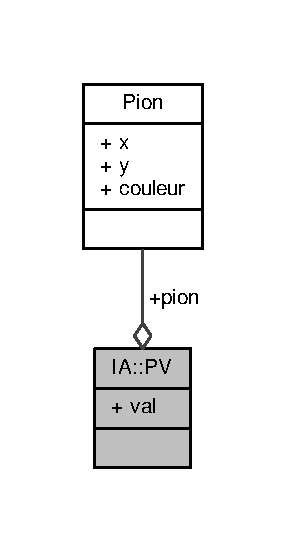
\includegraphics[width=137pt]{structIA_1_1PV__coll__graph}
\end{center}
\end{figure}
\subsection*{Attributs publics}
\begin{DoxyCompactItemize}
\item 
int {\bfseries val}\hypertarget{structIA_1_1PV_ad3a056627bcb61cbc44ea37f00ba6c6d}{}\label{structIA_1_1PV_ad3a056627bcb61cbc44ea37f00ba6c6d}

\item 
\hyperlink{structPion}{Pion} {\bfseries pion}\hypertarget{structIA_1_1PV_ad36e933f2e4936c2ed19138666c48859}{}\label{structIA_1_1PV_ad36e933f2e4936c2ed19138666c48859}

\end{DoxyCompactItemize}


La documentation de cette structure a été générée à partir du fichier suivant \+:\begin{DoxyCompactItemize}
\item 
ia.\+h\end{DoxyCompactItemize}

\hypertarget{classRandomIA}{}\section{Référence de la classe Random\+IA}
\label{classRandomIA}\index{Random\+IA@{Random\+IA}}


Graphe d\textquotesingle{}héritage de Random\+IA\+:\nopagebreak
\begin{figure}[H]
\begin{center}
\leavevmode
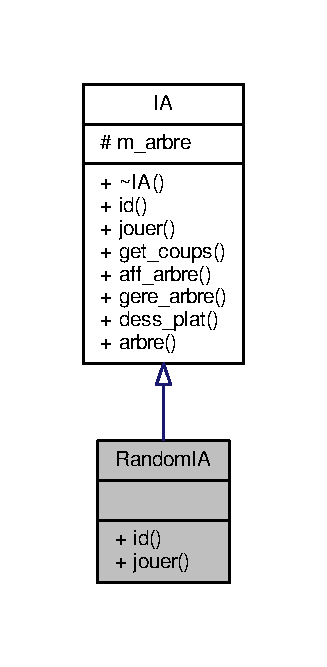
\includegraphics[width=157pt]{classRandomIA__inherit__graph}
\end{center}
\end{figure}


Graphe de collaboration de Random\+IA\+:\nopagebreak
\begin{figure}[H]
\begin{center}
\leavevmode
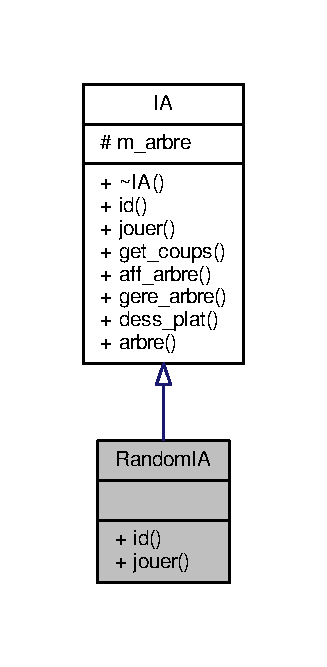
\includegraphics[width=157pt]{classRandomIA__coll__graph}
\end{center}
\end{figure}
\subsection*{Fonctions membres publiques}
\begin{DoxyCompactItemize}
\item 
virtual std\+::string \hyperlink{classRandomIA_a293e1635b96e7471cc105f0e421543db}{id} () const override\hypertarget{classRandomIA_a293e1635b96e7471cc105f0e421543db}{}\label{classRandomIA_a293e1635b96e7471cc105f0e421543db}

\begin{DoxyCompactList}\small\item\em Methode virtuel permetant de connaitre l\textquotesingle{}\hyperlink{classIA}{IA}. \end{DoxyCompactList}\item 
virtual \hyperlink{structPion}{Pion} \hyperlink{classRandomIA_a5e64b0d2e5ee8dcae31f4fbae8799dc3}{jouer} (\hyperlink{structEtat}{Etat} plateau) override\hypertarget{classRandomIA_a5e64b0d2e5ee8dcae31f4fbae8799dc3}{}\label{classRandomIA_a5e64b0d2e5ee8dcae31f4fbae8799dc3}

\begin{DoxyCompactList}\small\item\em Permet de générer les coups aléatoire en respectant les règles du jeu. \end{DoxyCompactList}\end{DoxyCompactItemize}
\subsection*{Membres hérités additionnels}


La documentation de cette classe a été générée à partir des fichiers suivants \+:\begin{DoxyCompactItemize}
\item 
\hyperlink{randomia_8h}{randomia.\+h}\item 
randomia.\+cpp\end{DoxyCompactItemize}

\hypertarget{classTableau}{}\section{Référence de la classe Tableau}
\label{classTableau}\index{Tableau@{Tableau}}


Graphe de collaboration de Tableau\+:\nopagebreak
\begin{figure}[H]
\begin{center}
\leavevmode
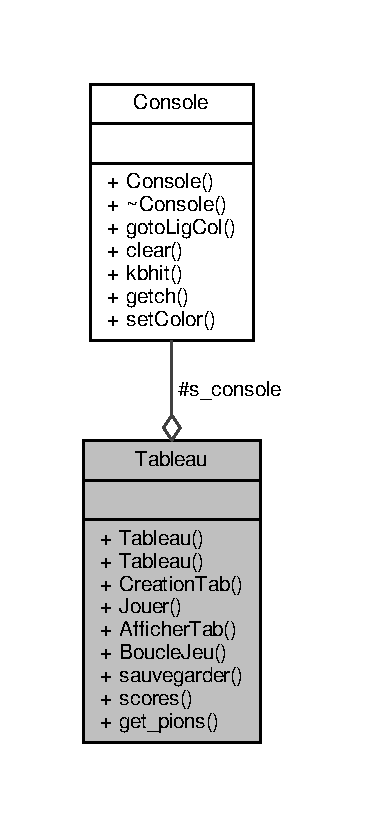
\includegraphics[width=176pt]{classTableau__coll__graph}
\end{center}
\end{figure}
\subsection*{Fonctions membres publiques}
\begin{DoxyCompactItemize}
\item 
{\bfseries Tableau} (std\+::shared\+\_\+ptr$<$ \hyperlink{classIA}{IA} $>$ ia\+\_\+noir=nullptr, std\+::shared\+\_\+ptr$<$ \hyperlink{classIA}{IA} $>$ ia\+\_\+blanc=nullptr)\hypertarget{classTableau_a4b7923326eb0e5e2d1d2f8acf6445545}{}\label{classTableau_a4b7923326eb0e5e2d1d2f8acf6445545}

\item 
{\bfseries Tableau} (\hyperlink{structEtat}{Etat} \&\&etat, std\+::shared\+\_\+ptr$<$ \hyperlink{classIA}{IA} $>$ ia\+\_\+noir, std\+::shared\+\_\+ptr$<$ \hyperlink{classIA}{IA} $>$ ia\+\_\+blanc)\hypertarget{classTableau_adc95e4c3d822d09af273e29294313ac4}{}\label{classTableau_adc95e4c3d822d09af273e29294313ac4}

\item 
void {\bfseries Creation\+Tab} ()\hypertarget{classTableau_a8e8311ab52129da568acc092598b22c7}{}\label{classTableau_a8e8311ab52129da568acc092598b22c7}

\item 
bool {\bfseries Jouer} (int \&x, int \&y)\hypertarget{classTableau_a564072da82e057d02ad7edbee98e6e43}{}\label{classTableau_a564072da82e057d02ad7edbee98e6e43}

\item 
void {\bfseries Afficher\+Tab} ()\hypertarget{classTableau_a422f7b27c74ca34d81ef3446e0d88bb7}{}\label{classTableau_a422f7b27c74ca34d81ef3446e0d88bb7}

\item 
C\+O\+U\+L\+E\+UR {\bfseries Boucle\+Jeu} ()\hypertarget{classTableau_aae276afa0929c10f4c9a37c61a6166a9}{}\label{classTableau_aae276afa0929c10f4c9a37c61a6166a9}

\item 
bool {\bfseries sauvegarder} () const \hypertarget{classTableau_a7fe5d033577a970525067422053595ba}{}\label{classTableau_a7fe5d033577a970525067422053595ba}

\item 
std\+::map$<$ C\+O\+U\+L\+E\+UR, unsigned $>$ const {\bfseries scores} () const \hypertarget{classTableau_ac3c035ec5fcc5189b04392ff56d0441e}{}\label{classTableau_ac3c035ec5fcc5189b04392ff56d0441e}

\item 
std\+::vector$<$ std\+::shared\+\_\+ptr$<$ \hyperlink{structPion}{Pion} $>$ $>$ const \& {\bfseries get\+\_\+pions} () const \hypertarget{classTableau_a41e9e9c45b4dfea82cf2c4bb64fdf5a6}{}\label{classTableau_a41e9e9c45b4dfea82cf2c4bb64fdf5a6}

\end{DoxyCompactItemize}
\subsection*{Attributs protégés}
\begin{DoxyCompactItemize}
\item 
\hyperlink{classConsole}{Console} $\ast$ {\bfseries s\+\_\+console} = N\+U\+LL\hypertarget{classTableau_a2557f30daf3e8c13d803b3365be83a64}{}\label{classTableau_a2557f30daf3e8c13d803b3365be83a64}

\end{DoxyCompactItemize}


La documentation de cette classe a été générée à partir des fichiers suivants \+:\begin{DoxyCompactItemize}
\item 
plateau.\+h\item 
plateau.\+cpp\end{DoxyCompactItemize}

\chapter{Documentation des fichiers}
\hypertarget{alphabetaia_8h}{}\section{Référence du fichier alphabetaia.\+h}
\label{alphabetaia_8h}\index{alphabetaia.\+h@{alphabetaia.\+h}}


\+: Défini \hyperlink{classAlphaBetaIA}{Alpha\+Beta\+IA} une \hyperlink{classIA}{IA} basée sur l\textquotesingle{}algorithme Alpha\+Beta  


{\ttfamily \#include $<$string$>$}\\*
{\ttfamily \#include \char`\"{}minmaxia.\+h\char`\"{}}\\*
Graphe des dépendances par inclusion de alphabetaia.\+h\+:\nopagebreak
\begin{figure}[H]
\begin{center}
\leavevmode
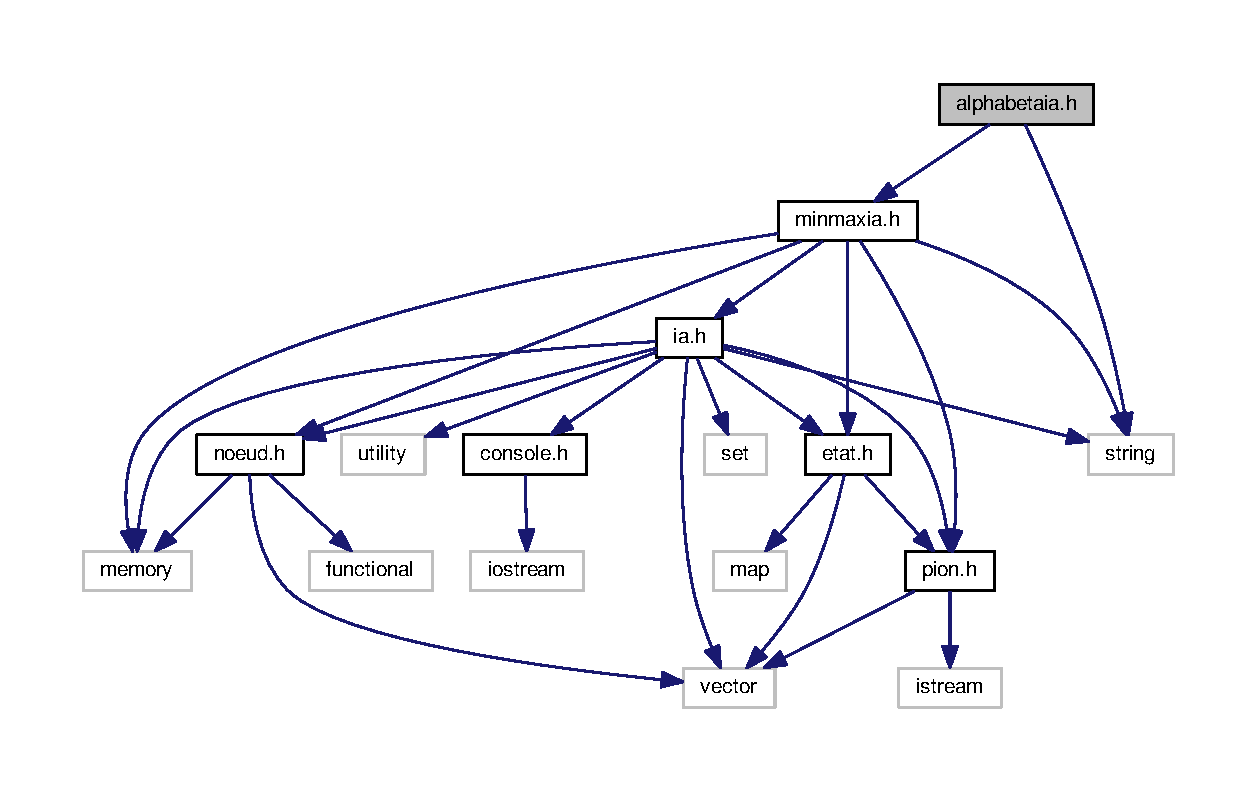
\includegraphics[width=350pt]{alphabetaia_8h__incl}
\end{center}
\end{figure}
Ce graphe montre quels fichiers incluent directement ou indirectement ce fichier \+:\nopagebreak
\begin{figure}[H]
\begin{center}
\leavevmode
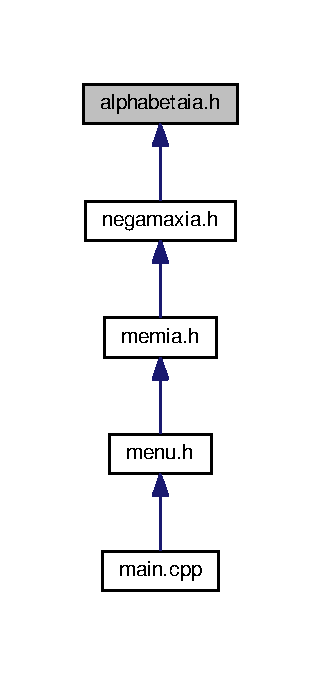
\includegraphics[width=154pt]{alphabetaia_8h__dep__incl}
\end{center}
\end{figure}
\subsection*{Classes}
\begin{DoxyCompactItemize}
\item 
class \hyperlink{classAlphaBetaIA}{Alpha\+Beta\+IA}
\end{DoxyCompactItemize}


\subsection{Description détaillée}
\+: Défini \hyperlink{classAlphaBetaIA}{Alpha\+Beta\+IA} une \hyperlink{classIA}{IA} basée sur l\textquotesingle{}algorithme Alpha\+Beta 

Pour plus d\textquotesingle{}explication sur l\textquotesingle{}algorithme suivez ce lien \+: \href{https://fr.wikipedia.org/wiki/%C3%89lagage_alpha-b%C3%AAta}{\tt https\+://fr.\+wikipedia.\+org/wiki/\%\+C3\%89lagage\+\_\+alpha-\/b\%\+C3\%\+A\+Ata} 
\hypertarget{etat_8h}{}\section{Référence du fichier etat.\+h}
\label{etat_8h}\index{etat.\+h@{etat.\+h}}
{\ttfamily \#include $<$map$>$}\\*
{\ttfamily \#include $<$vector$>$}\\*
{\ttfamily \#include \char`\"{}pion.\+h\char`\"{}}\\*
Graphe des dépendances par inclusion de etat.\+h\+:\nopagebreak
\begin{figure}[H]
\begin{center}
\leavevmode
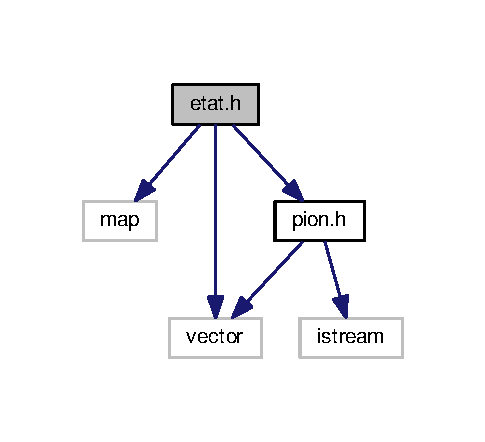
\includegraphics[width=233pt]{etat_8h__incl}
\end{center}
\end{figure}
Ce graphe montre quels fichiers incluent directement ou indirectement ce fichier \+:\nopagebreak
\begin{figure}[H]
\begin{center}
\leavevmode
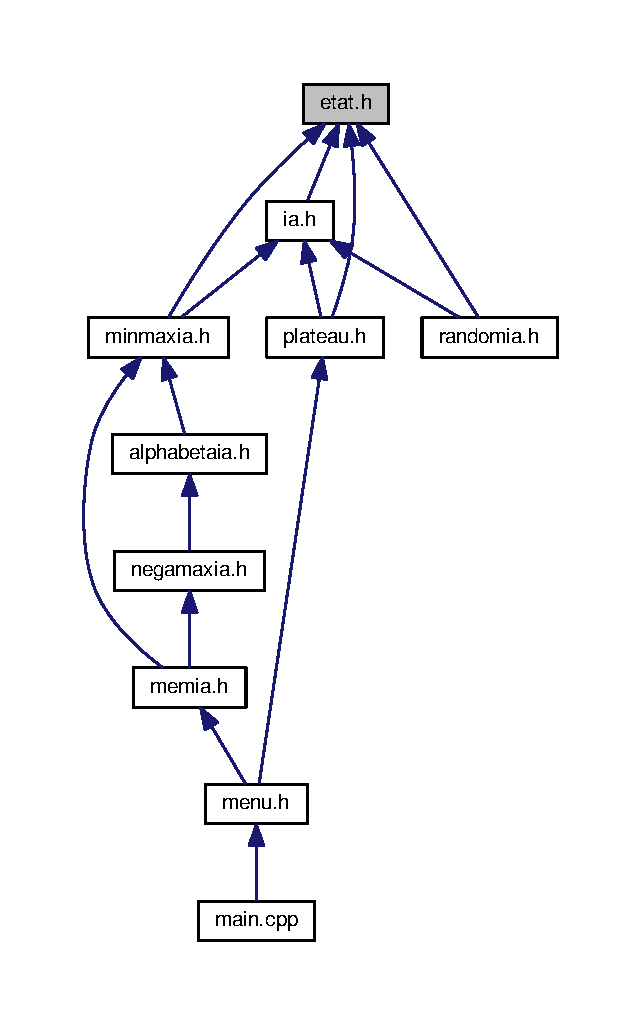
\includegraphics[width=308pt]{etat_8h__dep__incl}
\end{center}
\end{figure}
\subsection*{Classes}
\begin{DoxyCompactItemize}
\item 
struct \hyperlink{structEtat}{Etat}
\end{DoxyCompactItemize}


\subsection{Description détaillée}
La structure \hyperlink{structEtat}{Etat} ... Représente l\textquotesingle{}état actuel du jeu, utile pour les sauvegardes, (un historique ?) mais surtout pour l\textquotesingle{}\hyperlink{classIA}{IA} !

Vous faites ce que vous voulez ... mais l\textquotesingle{}\hyperlink{classIA}{IA} prendra cette structure en entrée ! 
\hypertarget{main_8cpp}{}\section{Référence du fichier main.\+cpp}
\label{main_8cpp}\index{main.\+cpp@{main.\+cpp}}
{\ttfamily \#include \char`\"{}menu.\+h\char`\"{}}\\*
Graphe des dépendances par inclusion de main.\+cpp\+:\nopagebreak
\begin{figure}[H]
\begin{center}
\leavevmode
\includegraphics[width=350pt]{main_8cpp__incl}
\end{center}
\end{figure}
\subsection*{Fonctions}
\begin{DoxyCompactItemize}
\item 
int {\bfseries main} ()\hypertarget{main_8cpp_ae66f6b31b5ad750f1fe042a706a4e3d4}{}\label{main_8cpp_ae66f6b31b5ad750f1fe042a706a4e3d4}

\end{DoxyCompactItemize}


\subsection{Description détaillée}
Petite note \+: ne jamais ajouter le dossier qt ! Y a un autre main dedans 
%--- End generated contents ---

% Index
\backmatter
\newpage
\phantomsection
\clearemptydoublepage
\addcontentsline{toc}{chapter}{Index}
\printindex

\end{document}
